\documentclass[11pt]{article}
\usepackage{report}
%\usepackage[swedish]{report} % Uncomment this if your report is in swedish.

\begin{document}
\tableofcontents

\clearpage
\section{Introduction}
\label{sec:introduction}
Lorem ipsum\footnote{wow} dolor sit amet, consectetuer adipiscing elit. Ut purus elit,
vestibulum ut, placerat ac, adipiscing vitae, felis. Curabitur dictum gravida
mauris. Nam arcu libero, nonummy eget, consectetuer id, vulputate a, magna.
Donec vehicula augue eu neque. Pellentesque habitant morbi tristique senectus
et netus et malesuada fames ac turpis egestas. Mauris ut leo\cite{example}.

\begin{figure}[hpb]
  \centering
  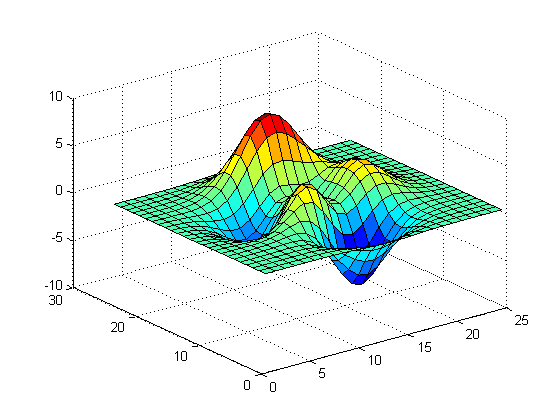
\includegraphics[width=0.7\textwidth]{example-plot.png}
  \caption{An example plot (see code in \cref{sec:appendix}).}
  \label{fig:plot}
\end{figure}

\begin{figure}[hpb]
  \centering
  \begin{subfigure}[b]{0.3\textwidth}
    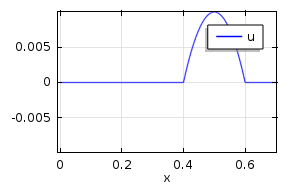
\includegraphics[width=\textwidth]{example-subplot1.png}
  \end{subfigure}
  \begin{subfigure}[b]{0.3\textwidth}
    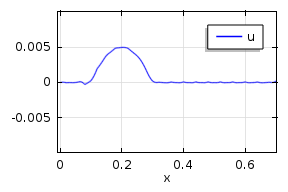
\includegraphics[width=\textwidth]{example-subplot2.png}
  \end{subfigure}
  \begin{subfigure}[b]{0.3\textwidth}
    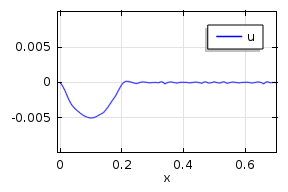
\includegraphics[width=\textwidth]{example-subplot3.png}
  \end{subfigure}
  \caption{Example of subfigures.}
\end{figure}

\clearpage
\section{Theory}
\label{sec:theory}

\begin{equation}
  \pd[2]{f}{x} + \pd{f}{x} = 0
\end{equation}

\clearpage
\section{Method}
\label{sec:method}

\clearpage
\section{Results}
\label{sec:results}

\clearpage
\section{Conclusion}
\label{sec:conclusion}

\clearpage
\begin{thebibliography}{9}

  \bibitem{example}
    Prime N Umber,
    \emph{Some Title}.
    Publisher, Location
    2014.

\end{thebibliography}

\clearpage
\appendix
\section{Appendix}
\label{sec:appendix}

\inputcode{example.m}
\inputcode[Python,caption=example.py]{example.py}

\end{document}
